\documentclass{article}

% if you need to pass options to natbib, use, e.g.:
% \PassOptionsToPackage{numbers, compress}{natbib}
% before loading nips_2017
%
% to avoid loading the natbib package, add option nonatbib:
% \usepackage[nonatbib]{nips_2017}

\usepackage{nips_2017}

% to compile a camera-ready version, add the [final] option, e.g.:
%\usepackage[final]{nips_2017}

%%%% PACKAGES TO USE
\usepackage[utf8]{inputenc} % allow utf-8 input
\usepackage[T1]{fontenc}    % use 8-bit T1 fonts
\usepackage{hyperref}       % hyperlinks
\usepackage{url}            % simple URL typesetting
\usepackage{booktabs}       % professional-quality tables
\usepackage{amsfonts}       % blackboard math symbols
\usepackage{nicefrac}       % compact symbols for 1/2, etc.
\usepackage{microtype}      % microtypography

%% Inigo
% Math related
\usepackage{amsmath}
% Indicator
\usepackage{bbm}
% Figures and subfigures
\usepackage{graphicx}
\usepackage{caption}
\usepackage{subcaption}
% Figures stay where told
\usepackage{float}
% Algorithms
\usepackage{algorithm}
\usepackage{algpseudocode}

%%%% DEFINITIONS-MACROS: Inigo
% Real line
\def \Real{{\mathbb R}} 
\def \Natural{{\mathbb N}} 
%Expected value
\newcommand{\eValue}[1]{\mathbb{E}\left\{ #1 \right\}}
% My small matrix
\newcommand{\mySmallMatrix}[1]{\left(\begin{smallmatrix} #1 \end{smallmatrix}\right)}
% Abbreviations
\newcommand{\ie}{i.e., }
\newcommand{\Ie}{I.e., }
\newcommand{\eg}{e.g. }
\newcommand{\Eg}{E.g. }
\newcommand{\etAl}{et al.\xspace}

%% Statistical-macros
%Distributions
\newcommand{\N}{\mathcal{N}}
\newcommand{\TN}{\mathcal{TN}}
\newcommand{\G}{\mathcal{G}}
\newcommand{\T}{\mathcal{T}}
\newcommand{\U}{\mathcal{U}}
\newcommand{\Dir}{{\rm Dir}}
\newcommand{\Cat}{{\rm Cat}}
\newcommand{\Mult}{{\rm Mult}}
\newcommand{\Bin}{{\rm Bin}}
\newcommand{\IG}{{\rm IG}}
\newcommand{\NIG}{{\rm NIG}}
\newcommand{\NIX}{{\rm NIX}}
\newcommand{\IW}{{\rm IW}}
\newcommand{\NIW}{{\rm NIW}}
\newcommand{\InvGa}{{\rm IG}}
\newcommand{\Chisquare}{\Chi^2}
\newcommand{\St}{{\rm St}}
\newcommand{\Beta}{{\rm Beta}}
\newcommand{\iid}{i.i.d. }
\newcommand{\Eta}{{\cal N}}
\newcommand{\Ber}{{\rm Ber}}

%Others
\newcommand{\ind}[1]{1_{#1}} % Indicator function
\newcommand{\pr}{P} % Generic probability
\newcommand{\var}{\textrm{Var}}
\newcommand{\cov}{\textrm{Cov}}
\newcommand{\sgn}{\textrm{sgn}}
\newcommand{\sign}{\textrm{sign}}
\newcommand{\kl}{\textrm{KL}} 
\newcommand{\abs}[1]{|{#1}|}
\newcommand{\Var}{\mathrm{Var}}
\newcommand{\Cov}{\mathrm{Cov}}
\newcommand{\tr}{\mathrm{tr}}
\newcommand{\diag}{\mathrm{diag}}
\newcommand{\deq}{:=}
\newcommand{\indep}{{\;\bot\!\!\!\!\!\!\bot\;}}
\newcommand{\eps}{\varepsilon}

\newcommand{\eqd}{\stackrel{d}{=}} % equal in distribution/law/measure
\newcommand{\argmax}{\mathop{\mathrm{argmax}}}
\newcommand{\argmin}{\mathop{\mathrm{argmin}}}
\newcommand{\conv}{\textrm{conv}} % for denoting the convex hull

%%%% Title and authors
\title{Bayesian bandits: balancing the exploration-exploitation tradeoff via double sampling}

% The \author macro works with any number of authors. There are two
% commands used to separate the names and addresses of multiple
% authors: \And and \AND.
%
% Using \And between authors leaves it to LaTeX to determine where to
% break the lines. Using \AND forces a line break at that point. So,
% if LaTeX puts 3 of 4 authors names on the first line, and the last
% on the second line, try using \AND instead of \And before the third
% author name.

\author{
	I\~{n}igo Urteaga\\
	Applied Physics and Applied Mathematics Department\\
	Data Science Institute\\
	Columbia University\\
	New York City, NY 10027\\
	\texttt{inigo.urteaga@columbia.edu} \\
	\And
	Chris H.~Wiggins\\
	Applied Physics and Applied Mathematics Department\\
	Data Science Institute\\
	Columbia University\\
	New York City, NY 10027\\
	\texttt{chris.wiggins@columbia.edu}
}

\begin{document}

\maketitle

\begin{abstract}
Reinforcement learning studies how to balance exploration and exploitation in real-world systems, optimizing interactions with the world while simultaneously learning how the world works. One general class of algorithms for such learning is the multi-armed bandit setting (in which sequential interactions are independent and identically distributed) and the related contextual bandit case, in which the distribution depends on different information or `context' presented with each interaction. Thompson sampling, though introduced in the 1930s, has recently been shown to perform well and to enjoy provable optimality properties, while at the same time permitting generative, interpretable modeling. In a Bayesian setting, prior knowledge is incorporated and the computed posteriors naturally capture the full state of knowledge. In several application domains, for example in health and medicine, each interaction with the world can be expensive and invasive, whereas drawing samples from the model is relatively inexpensive. Exploiting this viewpoint, we develop a double-sampling technique driven by the uncertainty in the learning process. It extends and out-performs (in the sense of regret) Thompson sampling. We illustrate using multi-armed bandit examples both with and without context.
\end{abstract}

\section{Introduction}
\label{sec:introduction}

In a plethora of problems in science and engineering, one needs to decide which action to take next based on partial information about the options available: a doctor must prescribe a medicine to a patient, a manager must allocate resources to competing projects, an ad serving algorithm must decide where to place ads, etc. In practice, the underlying properties of each choice are only partially known at the time of the decision, but one hopes that the understanding of the caveats involved will improve as time passes.

This set of problems has an illustrative gambling analogy, where a person facing a row of slot machines needs to devise its playing strategy (policy): which arms to play and in which order. Statisticians have studied this abstraction under the name of the multi-armed bandit problem for decades, e.g., in the seminal works by \cite{j-Robbins1956,j-Robbins1952}. Since then, it has played an important role in many fields across science and engineering.

Several algorithms have been proposed to overcome the exploration-exploitation tradeoff in such problems, mostly based on heuristics, on upper confidence bounds, or on the Gittins index. From the former, the $\epsilon$-greedy approach (randomly pick an arm with probability $\epsilon$, otherwise be greedy) has become very popular, due to its simplicity 
while nonetheless retaining often good performance (\cite{j-Auer2002}). In the latter case, \cite{j-Gittins1979} formulated a method based on computing the optimal strategy for some types of bandits, where geometrically discounted future rewards are considered. There are several difficulties inherent to the exact computation of the Gittins index and thus, approximations have been developed as well (\cite{j-Brezzi2002}). These and other intrinsic challenges of the method have limited its applicability (\cite{b-Sutton1998}). \cite{j-Lai1985} and \cite{j-Lai1987} introduced another class of algorithms, based on upper confidence intervals of the expected reward of each arm, for which strong theoretical guarantees were proved. Nevertheless, these algorithms might be far from optimal in the presence of dependent and more general reward distributions (\cite{j-Scott2010}).

More recently, the problem has re-emerged both from a practical (importance in e-commerce and web applications, \eg \cite{j-Li2010}) and a theoretical (research on probability matching algorithms and their regret bounds, \eg \cite{j-Agrawal2011} and \cite{ip-Maillard2011}) point of view. Contributing to this revival was the observation that
one of the oldest heuristics to address the exploration-exploitation trade-off, \ie \cite{j-Thompson1935,j-Thompson1933} sampling, has been empirically proven to perform satisfactorily (see \cite{ic-Chapelle2011} and \cite{j-Scott2015} for details). Contemporaneously, theoretical study established several performance bounds, both for problems with and without context (\cite{j-Agrawal2012,j-Agrawal2012a,ic-Korda2013,j-Russo2014,j-Russo2016}).

In this work, we are interested in the randomized probability matching approach, as it connects to the Bayesian learning paradigm which readily facilitates modeling and algorithm development in both sequential and batch processing scenarios. Specifically, we establish how one can extract more information about the environment by casting it as a Bayesian sequential learning problem, so that better informed decisions can be made, leading to a lower regret than in the Thompson sampling approach. Our motivation is cases where sampling from the model is inexpensive relative to interactions with the world, which may be expensive or invasive or, as in the medical application domain, both. We propose a technique that is based on Monte Carlo sampling (to approximate otherwise unsolvable integrals) and a sampling-based arm-selection policy. The policy is driven by the uncertainty in the learning process, as it favors exploitation when certain about the properties of each arm, exploring otherwise.

We formally introduce the problem in Section \ref{sec:problem_formulation}, before providing all the details of our proposed method, double sampling, in Section \ref{sec:proposed_method}. The performance of 
%our technique 
double sampling
is compared to the Thompson sampling approach in Section \ref{sec:evaluation}, and we conclude with final remarks in Section \ref{sec:conclusion}.

\section{Problem formulation}
\label{sec:problem_formulation}

We mathematically formulate the multi-armed bandit problem as follows. Let $a\in\{1,\cdots,A\}$ indicate the arms of the bandit (possible actions to take) and $f_{a}(y|\theta)$ the stochastic reward distribution of each arm. For every time instant, the observed reward $y_t$ is independently drawn from the reward distribution corresponding to the played arm. We denote $a_t$ as the arm played at time instant $t$; $a_{1:t} \equiv (a_1, \cdots , a_t)$ refers to the sequence of arms played, and similarly $y_{1:t} \equiv (y_1, \cdots , y_t)$ refers to the sequence of observed rewards up to time $t$.

In the multi-armed bandit setting one must decide, based on observed rewards $y_{1:t}$ and actions $a_{1:t}$, which arm to play next in order to maximize rewards. Due to the stochastic nature of the rewards, their expectation under the arm's distribution is the most common metric used. We denote each arm's expected reward as $\mu_{a}(\theta)=\mathbb{E}_{a}\{y|\theta\}$, which is parameterized by the arm-dependent parameters $\theta$. When the properties of the arms (\ie their parameters) are known, one can readily determine the optimal selection policy, \ie
		\begin{equation}
		a^*(\theta)=\argmax_{a}\mu_{a}(\theta) \; .
		\end{equation}
		
However, the optimal solution for the multi-armed bandit is only computable in closed form in very few special cases (\cite{j-Bellm1956, j-Gittins1979}), and it fails to generalize to more realistic reward distributions and scenarios (\cite{j-Scott2010}). The biggest challenge occurs when the parameters are unknown, as one might end up playing the wrong arm forever if incomplete learning occurs (\cite{j-Brezzi2000}). Practitioners have often turned to heuristics to overcome these issues, and amongst them, the randomized probability matching, \ie playing each arm in proportion to its probability of being optimal, is a particularly appealing one.

Given the parameters $\theta$, the expected reward of each arm is deterministic and, thus, one must pick the arm with the maximum expected reward
\begin{equation}
\mathrm{Pr}\left[a=a_{t+1}^*|a_{1:t}, y_{1:t}, \theta \right] = \mathrm{Pr}\left[a=a_{t+1}^*|\theta \right] = I_a(\theta) \;,
\end{equation}
where we use the indicator function
\begin{equation}
I_a(\theta) = \begin{cases}
1, \; \mu_{a}(\theta)=\max\{\mu_1(\theta), \cdots, \mu_A(\theta)\} \;, \\
0, \; \text{otherwise} \;.
\end{cases}
\label{eq:theta_known_pr_arm_optimal}
\end{equation}

Under random probability matching, the aim is to compute the probability of a given arm $a$ being optimal for the next time instant, $p_{a,t+1}\in [0,1]$, even with unknown parameters. Mathematically,
\begin{equation}
p_{a,t+1} \equiv \mathrm{Pr}\left[a=a_{t+1}^* \big| a_{1:t}, y_{1:t}\right]=\mathrm{Pr}\left[ \mu_{a}(\theta) = \max\{\mu_1(\theta), \cdots, \mu_A(\theta)\} \big| a_{1:t}, y_{1:t}\right].
\label{eq:theta_unknown_pr_arm_optimal}
\end{equation}

In this case, there is uncertainty about the unknown properties of the arms, as Eqn. \ref{eq:theta_unknown_pr_arm_optimal} is parameterized by $\theta$, while Eqn. \ref{eq:theta_known_pr_arm_optimal} is not. In order to compute a solution to this problem, recasting it as a Bayesian learning problem is of great help, as it allows for direct connection with the randomized probability matching technique (\cite{j-Scott2010}). The randomized probability matching approach has shown to be easy to implement, efficient and broadly applicable.

\section{Proposed method: double sampling}
\label{sec:proposed_method}

The multi-armed bandit problem consists of two separate but intertwined tasks: (1) learning about the properties of the arms, and (2) deciding what arm to play next. The problem is sequential in nature, as one makes a decision on which arm to play and learns from the observed reward, one observation at a time. We cast the multi-armed bandit problem as a sequential Bayesian learning task (\cite{b-Bernardo2009}). By doing so, we capture the full state of knowledge about the world at every time instant. We incorporate any available prior information to the learning process, and update our knowledge about the unknown parameters $\theta$, as we sequentially play arms and observe rewards. This learning can be done both sequentially or in batches, as Bayesian posterior updates are computable for both cases. However, the solution to the probability matching equation is analytically intractable, so we approximate it via Monte Carlo sampling. For balancing the exploration-exploitation tradeoff, we propose a sampling-based probability matching technique. 
The proposed arm-selection policy is a function of the uncertainty in the learning process. The intuition is that we exploit only when certain about the properties of the arms, while we keep exploring otherwise. We elaborate on the foundations of the proposed method in the following sections, before presenting the algorithm in \autoref{alg:bayesianDoubleSampling}.

\subsection{The Bayesian multi-armed bandit}
\label{ssec:bayesian_multi_armed_bandit}

We are interested in computing, after playing arms $a_{1:t}$ and observing rewards $y_{1:t}$, the probability of each arm $a$ being optimal for the next time instant, \ie
\begin{equation}
p_{a,t+1} \equiv \mathrm{Pr}\left[a=a_{t+1}^* \big| a_{1:t}, y_{1:t}\right]=\mathrm{Pr}\left[ \mu_{a}(\theta) = \max\{\mu_1(\theta), \cdots, \mu_A(\theta)\} \big| a_{1:t}, y_{1:t}\right] .
\end{equation}

In practice, one needs to account for the lack of knowledge of each arm's properties, \ie the unknown parameters $\theta$. We can do so by following the Bayesian methodology, where the parameters are considered to be another set of random variables. The uncertainty over the parameters can be accounted for by marginalizing over their probability distribution. Specifically, we marginalize over the posterior of the parameters after observing rewards and actions up to $t$
\begin{equation}
\begin{split}
p_{a,t+1} \equiv \mathrm{Pr}\left[a=a_{t+1}^* \big| a_{1:t}, y_{1:t}\right]&=f(a=a^*_{t+1}|a_{1:t}, y_{1:t}) =\int f(a|a_{1:t}, y_{1:t}, \theta) f(\theta|a_{1:t}, y_{1:t}) \mathrm{d}\theta \;.
\end{split}
\label{eq:pr_arm_optimal_bayes}
\end{equation}

Given a prior for the parameters $f(\theta)$ and the per-arm reward distribution $f_{a}(y|\theta)$, one can compute the posterior of each arm's parameters by
\begin{equation}
\begin{split}
f(\theta|a_{1:t}, y_{1:t}) &\propto f_{a_t}(y_t | \theta)f(\theta | a_{1:t-1}, y_{1:t-1}) = \left[\prod_{\tau=1}^t f_{a_{\tau}}(y_{\tau}|\theta)\right] f(\theta) \; .
\end{split}
\label{eq:seq_param_posterior}
\end{equation}

This posterior provides information (with uncertainty) about the state of the arm. In this work, we focus on the parameter posterior updates for two of the most studied (the Bernoulli and the contextual linear Gaussian) bandits. Note that the updates (provided later in subsection \ref{ssec:bernoulli_bandits} and subsection \ref{ssec:contextLinearGaussian_bandits}) can be written in both sequential and batch forms. This flexibility is of great help in many practical scenarios, as one can learn from historic data, as well as process data as it comes.

Even if analytical expressions for the parameter posteriors are available for many models of interest, computing the probability of any given arm being optimal is analytically intractable, due to the nonlinearities induced by the indicator function
\begin{equation}
\begin{split}
p_{a,t+1} \equiv f(a=a^*_{t+1}|a_{1:t}, y_{1:t})&=\int f(a|a_{1:t}, y_{1:t}, \theta) f(\theta|a_{1:t}, y_{1:t}) \mathrm{d}\theta = \int I_a(\theta) f(\theta|a_{1:t}, y_{1:t}) \mathrm{d}\theta \; .
\label{eq:pr_arm_optimal_bayes_indicator}
\end{split}
\end{equation}

\subsection{Monte-Carlo integration}
\label{ssec:mc_integration}

We harness the power of Monte Carlo sampling to compute the otherwise analytically intractable integral for $p_{a,t+1}\in [0,1]$ in Eqn. \ref{eq:pr_arm_optimal_bayes_indicator}. We obtain its Monte Carlo approximation as follows:
\begin{enumerate}
	\item Draw $M$ parameter samples from the updated posterior distribution
	\begin{equation}
	\theta^{(m)}\sim f(\theta|a_{1:t}, y_{1:t}), \; m=\{1, \cdots, M\} \; .
	\end{equation}
	\item For each parameter sample $\theta^{(m)}$, compute the expected reward and determine the best arm 
	\begin{equation}
	a_{t+1}^*(\theta^{(m)})=\argmax_{a}\mu_{a}(\theta^{(m)}) \; .
	\end{equation}
	\item Define the random measure approximation to the probability distribution in Eqn. \ref{eq:pr_arm_optimal} as
	\begin{equation}
	f_M(a =a_{t+1}^*|a_{1:t}, y_{1:t}) = \frac{1}{M} \sum_{m=1}^M \delta\left(a - a_{t+1}^*(\theta^{(m)}) \right) \; ,
	\label{eq:pr_arm_optimal_bayes_MC}
	\end{equation}
	where $\delta(\cdot)$ denotes the Dirac delta function.
	\item Estimate the first- and second-order sufficient statistics of the distribution
	\begin{equation}
	\begin{cases}
	\hat{p}_{a,t+1}=\frac{1}{M}\sum_{m=1}^M I_a\left(\theta^{(m)}\right) \; , \\
	\hat{\sigma}^2_{a,t+1}=\frac{1}{M} \sum_{m=1}^M \left(I_a\left(\theta^{(m)}\right)- \hat{p}_{a,t+1} \right)^2 \; .
	\end{cases}
	\label{eq:pr_arm_optimal_bayes_MC_suff_statistics}
	\end{equation}
	\item Estimate which is the optimal arm and with what probability
	\begin{equation}
	\begin{cases}
	\hat{a}_{t+1}^* =\argmax_{a} \hat{p}_{a,t+1} \; ,  \\
	\hat{p}^*_{a,t+1}=\max_{a} \hat{p}_{a,t+1} \; .
	\end{cases}
	\end{equation}
\end{enumerate}

\subsection{Sampling-based policy}
\label{ssec:sampling_policy}

Given the available information at any given time $t$, one needs to decide which arm to play next. A randomized probability matching technique would pick the next arm $a$ with probability $p_{a,t+1}$. On the contrary, a greedy approach would choose the arm with the highest probability of being optimal (\ie $p^*_{a,t+1}$). We present an alternative sampling-based probability matching arm-selection policy that automatically finds a balance between these two cases. We rely on the Monte Carlo approximation to Eqn. \ref{eq:pr_arm_optimal_bayes_indicator}, and leverage the estimated sufficient statistics in Eqn. \ref{eq:pr_arm_optimal_bayes_MC_suff_statistics} to balance the exploration-exploitation tradeoff. 

We draw candidate arm samples from the random measure in Eqn. \ref{eq:pr_arm_optimal_bayes_MC}, and automatically adjust the probability matching technique according to the accuracy of this approximation. We account for the uncertainty of the learning process in the arm-selection policy, dynamically balancing exploration and exploitation. The number of candidate arm samples drawn is instrumental for our sampling based policy. We automatically adjust its value according to the uncertainty on the optimality of each arm (\ie $\hat{\sigma}^2_{a,t+1}$).

The number of candidate arm samples to draw is inversely proportional to the probability of not picking the optimal arm. We denote this probability as $p_{FA}$, which is computed for each arm as
\begin{equation}
p_{FA}^{(a)} =Pr\left(p_{a,t+1} > p^*_{a,t+1} \right) = 1 - F_{p_{a,t+1}}(p^*_{a,{t+1}}) \; ,
\end{equation}
where $p_{a,t+1}^*=\max_{a}p_{a,t+1}$. Since we can not exactly evaluate $p_{a,t+1}$, we resort to our Monte Carlo estimates in Eqn. \ref{eq:pr_arm_optimal_bayes_MC_suff_statistics}. The true cumulative density function $F_{p_{a,t+1}}(\cdot)$ is analytically intractable as well, but we approximate it with a truncated Gaussian
\begin{equation}
F_{p_{a,t+1}}(p^*_{a,{t+1}}) \approx \Phi_{[0,1]}\left(\frac{\hat{p}_{a,t+1} - \hat{p}^*_{a,{t+1}}}{\hat{\sigma}_{a,t+1}}\right) \;.
\end{equation}

The proposed sampling policy proceeds as follows:
\begin{enumerate}
	\item Determine $N_{t+1}$, the number of candidate arm samples to draw
		\begin{equation}
		N_{t+1} \propto \log\left(\frac{1}{p_{FA}}\right), \; p_{FA}=\frac{1}{K-1}\sum_{a \neq \hat{a}_{t+1}^*}p_{FA}^{(a)}\;, \; p_{FA}^{(a)} \approx 1- \Phi_{[0,1]}\left(\frac{\hat{p}_{a,t+1} - \hat{p}^*_{a,{t+1}}}{\hat{\sigma}_{a,t+1}}\right) \; .
		\label{eq:policy_n_samples}
		\end{equation}
	\item Draw $N_{t+1}$ candidate arm samples from the random measure in Eqn. \ref{eq:pr_arm_optimal_bayes_MC}
	\begin{equation}
	\hat{a}_{t+1}^{(n)} \sim \Cat \left(\hat{p}_{a,t+1}\right) \; , \qquad n=1,\cdots, N_{t+1} \; .
	\end{equation}
	\item Pick the most probable optimal arm, given drawn candidate arm samples $\hat{a}_{t+1}^{(n)}$
	\begin{equation}
	a_{t+1} = \text{Mode}\left(\hat{a}_{t+1}^{(n)}\right) \; , \qquad  n=1,\cdots,N_{t+1} \;.
	\end{equation}
\end{enumerate}

By allowing for $N_{t+1}$ to be adjusted based upon the uncertainty of the learning process, we balance the exploration-exploitation tradeoff. The proposed sampling policy reduces to a probabilistic matching regime when uncertain about the arms, (\ie $N_t \approx 1$), but favors exploitation ($N_t \gg 1$) when the probability of picking a suboptimal arm is low. In other words, double sampling exploits only when confident about the learned probabilities ($\hat{\sigma}_{a,t+1} \rightarrow 0, N \gg 1)$, and picks the arm with the highest probability $\hat{p}_{a,t+1}$. However, for $N_t \approx 1$, a randomized probability matching is in play. Note that Thompson sampling is a special case of double sampling, when $N_{t}=1 \;, \forall t$.

%Bayesian Double Sampling Algorithm
\begin{algorithm}
	\begin{algorithmic}
		\Require Number of arms $A$
		\Require Prior over model parameters $f(\theta)$
		\Require Per-arm reward distributions $f_a(y|\theta)$
		\Require Horizon $T$
		\State $D=\emptyset$
		\For{$t=1, \cdots, T$}
		\State Draw $M$ parameter samples from the updated posterior distribution
		\begin{equation}
		\theta_{t+1}^{(m)}\sim f(\theta|a_{1:t}, y_{1:t}), \; m=\{1, \cdots, M\} \; .
		\end{equation}
		\State If applicable, receive context $x_{t+1}$
		\For{$a=1, \cdots, A$}
		\State Compute the expected reward for each parameter sample $\theta_{t+1}^{(m)}$
		\begin{equation}
		\mu_{a,t+1}(\theta_{t+1}^{(m)})=\mu_{a}(x_{t+1},\theta_{t+1}^{(m)})=\mathbb{E}_{a}\{y|x_{t+1},\theta_{t+1}^{(m)}\}
		\end{equation}
		\State Compute the first- and second-order sufficient statistics of each arm being optimal
		\begin{equation}
		\begin{split}
		&\begin{cases}
		\hat{p}_{a,t+1}=\frac{1}{M}\sum_{m=1}^M I_a\left(\theta_{t+1}^{(m)}\right) \; , \\
		\hat{\sigma}^2_{a,t+1}=\frac{1}{M} \sum_{m=1}^M \left(I_a\left(\theta_{t+1}^{(m)}\right)- \hat{p}_{a,t+1} \right)^2 \; ,
		\end{cases} \\
		&\text{ where }I_a(\theta_{t+1}^{(m)}) = \begin{cases}
		1, \; \mu_{a}(\theta_{t+1}^{(m)})=\max\{\mu_1(\theta_{t+1}^{(m)}), \cdots, \mu_A(\theta_{t+1}^{(m)})\} \;, \\
		0, \; \text{otherwise} \;.
		\end{cases}
		\end{split}
		\end{equation}
		\EndFor
		\State Estimate the optimal arm and its probability of being optimal
		\begin{equation}
		\begin{cases}
		\hat{a}_{t+1}^* =\argmax_{a} \hat{p}_{a,t+1} \; ,  \\
		\hat{p}^*_{a,t+1}=\max_{a} \hat{p}_{a,t+1} \; .
		\end{cases}
		\end{equation}
		\For{$a=1,\cdots, A$}
		\State Compute the estimated probability of each arm not being the optimal arm
		\begin{equation}
		\begin{split}
		\hat{p}_{FA}^{(a)} =Pr\left(\hat{p}_{a,t+1} > \hat{p}^*_{a,t+1} \right) &= 1 - F_{\hat{p}_{a,t+1}}(\hat{p}^*_{a,{t+1}}) \; , \\
		F_{\hat{p}_{a,t+1}}(p^*_{a,{t+1}}) &\approx \Phi_{[0,1]}\left(\frac{\hat{p}_{a,t+1} - \hat{p}^*_{a,{t+1}}}{\hat{\sigma}_{a,t+1}}\right) \;.
		\end{split}
		\end{equation}
		\EndFor
		\State Compute $N_{t+1}$, the number of candidate arm samples to draw
		\begin{equation}
		N_{t+1} \propto \log\left(\frac{1}{\hat{p}_{FA}}\right), \; \hat{p}_{FA}=\frac{1}{A-1}\sum_{a \neq \hat{a}_{t+1}^*}\hat{p}_{FA}^{(a)}\; .
		\end{equation}
		\State Draw $N_{t+1}$ candidate arm samples
		\begin{equation}
		\hat{a}_{t+1}^{(n)} \sim \Cat \left(\hat{p}_{a,t+1}\right) \; , \qquad n=1,\cdots, N_{t+1} \; .
		\end{equation}
		\State Play arm
		\begin{equation}
		a_{t+1} = \text{Mode}\left(\hat{a}_{t+1}^{(n)}\right) \; , \qquad  n=1,\cdots,N_{t+1} \;.
		\end{equation}
		\State Observe reward $y_{t+1}$
		\State $D=D \cup \left\{x_{t+1}, a_{t+1}, y_{t+1}\right\}$
		\EndFor
	\end{algorithmic}
	\caption{Bayesian Double Sampling algorithm}
	\label{alg:bayesianDoubleSampling}
\end{algorithm}

\section{Evaluation: Thompson sampling vs. double sampling}
\label{sec:evaluation}

We now provide empirical evidence of our double sampling's lower regret relative to Thompson sampling. We consider both discrete and continuous multi-armed bandits, and the contextual setting as well. We compare the performance of our algorithm , as presented in \autoref{alg:bayesianDoubleSampling}, to that of Thompson sampling, for both the Bernoulli and the contextual linear Gaussian bandits. As is standard in the literature, we measure performance in the cumulative regret sense, \ie
\begin{equation}
R_t=\sum_{\tau=0}^t \eValue{\left(y^*_{\tau}-y_{\tau} \right)} = \sum_{\tau=0}^t \mu_\tau^*-\bar{y}_{\tau} \; ,
\end{equation}
where for each time instant $t$, $\mu_t^*$ denotes the expected reward of the optimal arm and $\bar{y}_{t}$ the empirical mean of the observed rewards.

\subsection{Bernoulli bandits}
\label{ssec:bernoulli_bandits}

Bernoulli bandits are well suited for applications with binary rewards (\ie success or failure of an action). The rewards of each arm are modeled as independent draws from a Bernoulli distribution with success probabilities $\theta_a$, \ie
\begin{equation}
f_a(y|\theta)=\theta_a^{y}(1-\theta_a)^{(1-y)} \; .
\end{equation}
For this reward distribution, the posterior parameter update can be computed using the conjugate prior distribution $f(\theta_a|\alpha_{a,0}, \beta_{a,0})=\Beta(\theta_a|\alpha_{a,0}, \beta_{a,0})$. After observing actions $a_{1:t}$ and rewards $y_{1:t}$, the posterior parameter distribution follows an updated Beta distribution
\begin{equation}\begin{split}
&f(\theta_a|a_{1:t}, y_{1:t}, \alpha_{a,0}, \beta_{a,0}) =f(\theta_a|\alpha_{a,t}, \beta_{a,t})=\Beta(\theta_a|\alpha_{a,t}, \beta_{a,t})  \; ,\\
\text{with} & \begin{cases}
\text{sequential updates} \begin{cases}
\alpha_{a,t}=\alpha_{a,t-1} + y_{t} \cdot \mathbbm{1}[a_t=a]\\
\beta_{a,t}=\beta_{a,t-1} + (1 - y_{t}) \cdot \mathbbm{1}[a_t=a]
\end{cases} \\
\text{batch updates} \qquad \begin{cases}
\alpha_{a,t}=\alpha_{a,0} + \sum_{t|a_t=a} y_{t} \\
\beta_{a,t}=\beta_{a,0} + \sum_{t|a_t=a} (1-y_{t}).
\end{cases}
\end{cases}
\end{split}
\end{equation}

We dissect the key aspects of double sampling in a particular realization of a three-armed Bernoulli bandit with parameters $\theta=\left(0.4 \; 0.7 \; 0.8 \right)$. The sequential Bayesian learning process is illustrated in Fig. \ref{fig:pred_action_density}, where we show the evolution of the probability of each arm being optimal (\ie the Monte Carlo approximation in Eqn. \ref{eq:pr_arm_optimal_bayes_MC}). For all results to follow, Monte Carlo integration is attained with $M=1000$ samples, as larger $M$s do not significantly improve regret performance. In Fig. \ref{fig:n_samples}, we illustrate how double sampling is {\em automatically} adjusted according to the learning process uncertainty, via the number of arm samples to draw (\ie $N_{t+1}$ in Eqn. \ref{eq:policy_n_samples}).

% Computed sufficient statistics and sampling policy N_{t+1}
\begin{figure}[!h]
	\centering
	\begin{subfigure}[b]{0.33\textwidth}
		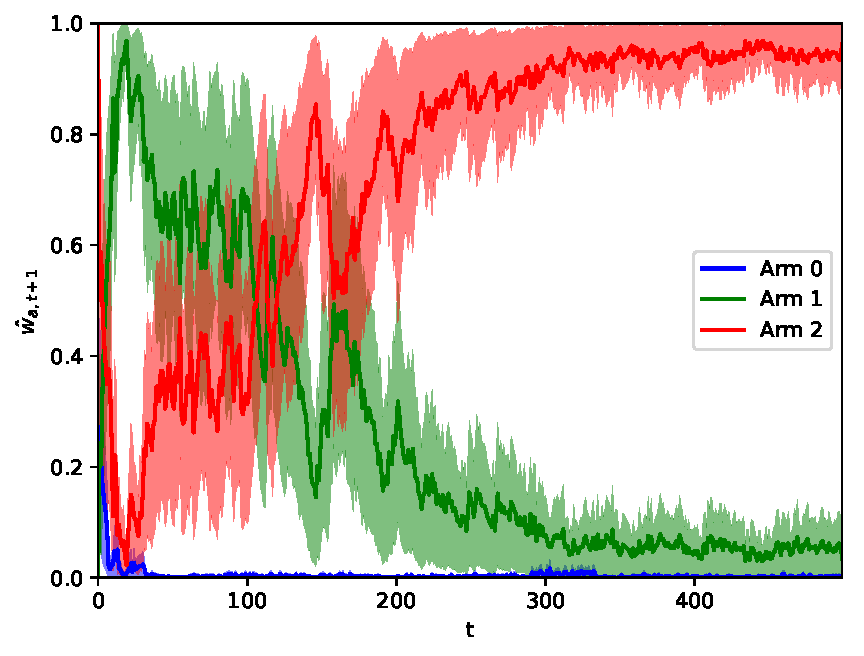
\includegraphics[width=\textwidth]{./figs/bernoulli/pred_action_density.pdf}
		\caption{Approximation to $w_{a,t+1}$.}
		\label{fig:pred_action_density}
	\end{subfigure}%
	%add desired spacing between images, e. g. ~, \quad, \qquad etc.
	%(or a blank line to force the subfigure onto a new line)
	\begin{subfigure}[b]{0.33\textwidth}
		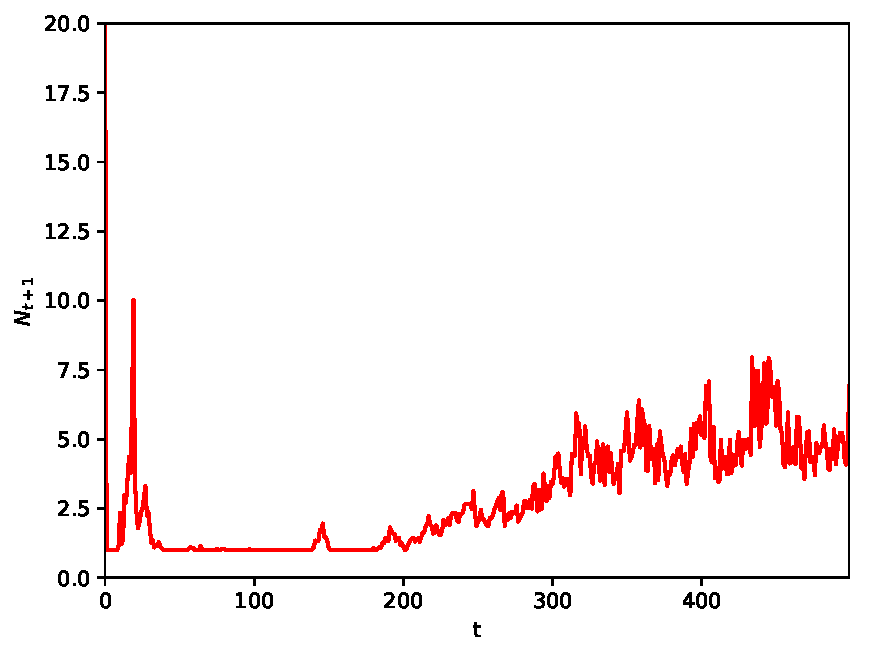
\includegraphics[width=\textwidth]{./figs/bernoulli/n_samples.pdf}
		\caption{Number of arm samples $N_{t+1}$.}
		\label{fig:n_samples}
	\end{subfigure}
	\begin{subfigure}[b]{0.33\textwidth}
		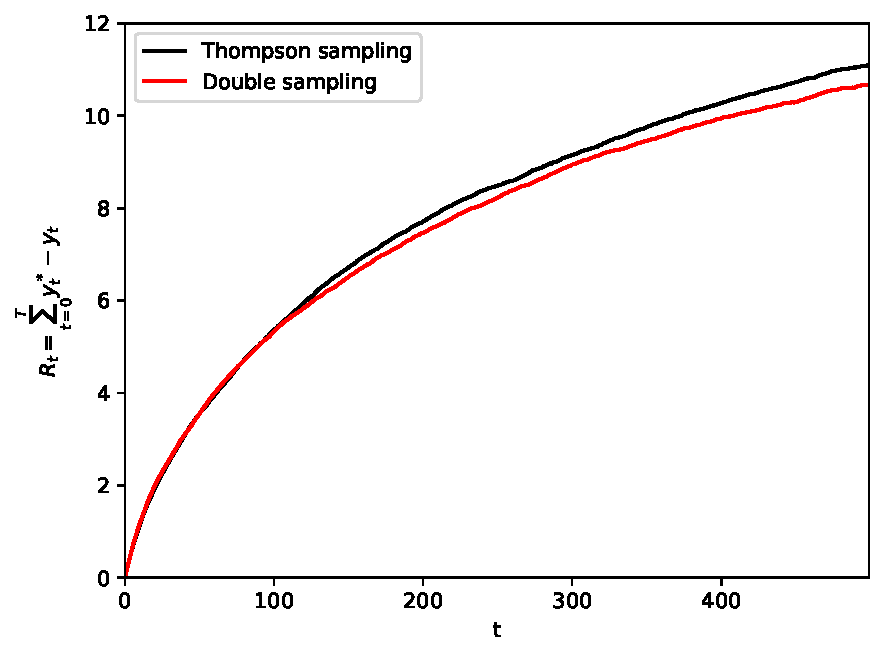
\includegraphics[width=\textwidth]{./figs/bernoulli/cumulative_regret.pdf}
		\caption{Averaged cumulative regret.}
		\label{fig:cumulative_regret}
	\end{subfigure}
	\caption{Empirical results with double sampling.}
	\label{fig:approach_intuition}
\end{figure}

For the case shown in Fig. \ref{fig:approach_intuition}, arm 0 (with $\theta_0=0.4$) is quickly discarded as being optimal, while the decision over which of the other two arms is better requires further learning. For some time ($t<200$), there is high uncertainty about the properties of both arms (high variance in Fig. \ref{fig:pred_action_density}). Thus, double sampling favors exploration ($N_{t+1}\approx 1$ in Fig. \ref{fig:n_samples}), until the uncertainty about which arm is best is reduced. Once the algorithm becomes more certain about the better reward properties of arm 2 ($t>200$), the sampling approach gradually favors a greedier policy ($N_{t+1}>1$). As a result, the cumulative regret of our proposed technique is reduced when compared to the Thompson sampling approach (see averaged cumulative regrets in Fig. \ref{fig:cumulative_regret}). All the averaged results presented in this paper are computed over 5000 realizations of the same set of parameters.

In Fig. \ref{fig:bernoulli_cumulative_regret_compare}, we show two antagonistic examples of the performance of double sampling. Our algorithm provides a clear benefit over Thompson sampling in Fig. \ref{fig:bernoulli_cumulative_regret_great}, though it performs only slightly better than Thompson sampling in Fig. \ref{fig:bernoulli_cumulative_regret_notgreat}. Such a cumulative regret difference is explained by the unknown nature of the bandit's arms. When the properties of the arms are very similar to each other, our algorithm resorts to a Thompson sampling-like policy ($N_{t+1}\approx1$), yielding near-equivalent sampling (and thus regret). However, when the learning process is certain about the properties of the arms, double sampling can considerably reduce the method's cumulative regret. Mathematically, the difference in arm properties can be captured by the divergence between their respective reward distributions. By computing the minimum Kullback-Leibler (KL) divergence between arms, we get an insight onto how ``difficult'' a multi-armed bandit problem is.

% Bernoulli: comparison of cumulative regret cases
\begin{figure}[!h]
	\centering
	\begin{subfigure}[b]{0.5\textwidth}
		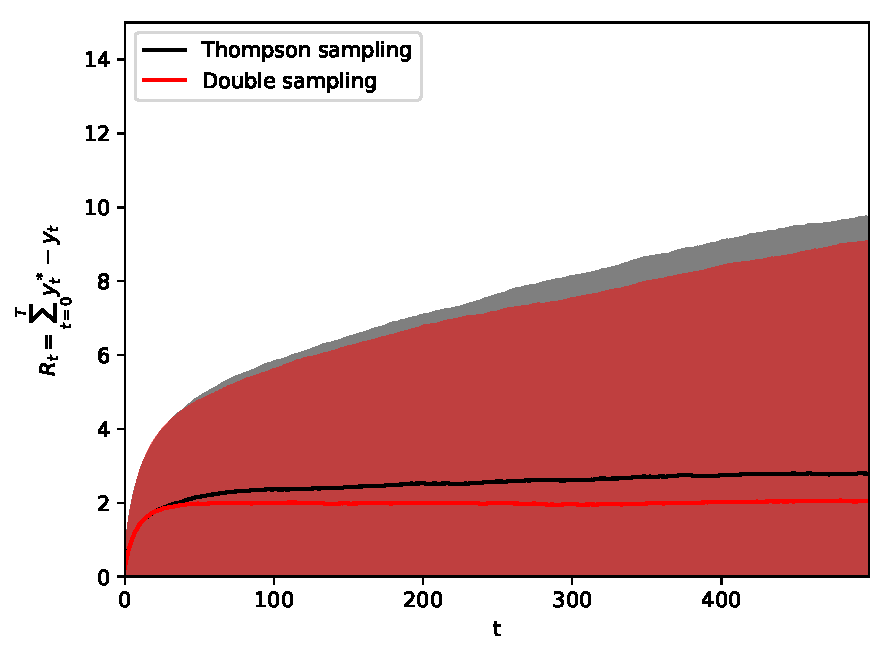
\includegraphics[width=\textwidth]{./figs/bernoulli/cumulative_regret_great.pdf}
		\caption{Cumulative regret with $A=2, \theta=\left(0.4 \; 0.9\right)$.}
		\label{fig:bernoulli_cumulative_regret_great}
	\end{subfigure}%
	%add desired spacing between images, e. g. ~, \quad, \qquad etc.
	%(or a blank line to force the subfigure onto a new line)
	\begin{subfigure}[b]{0.5\textwidth}
		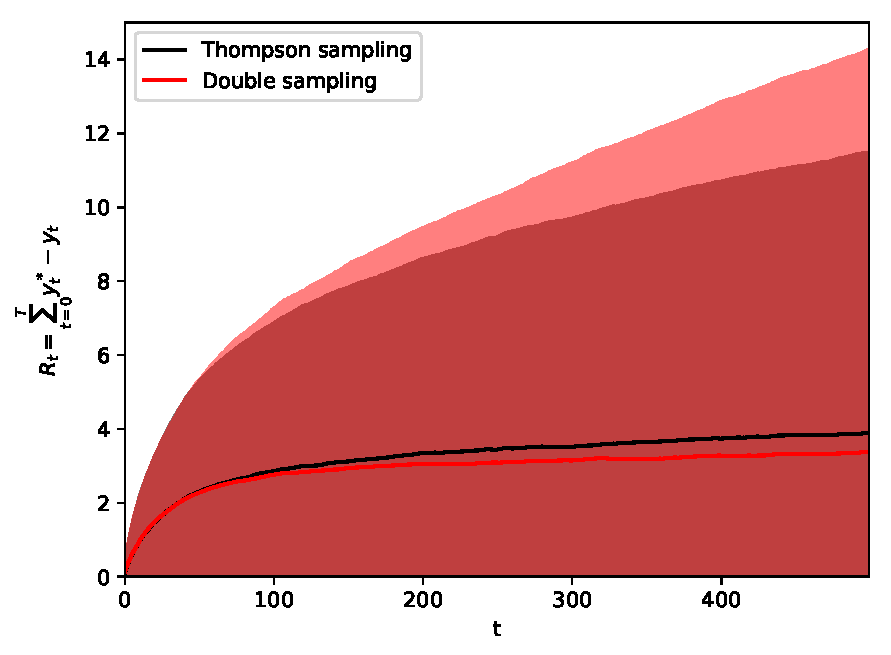
\includegraphics[width=\textwidth]{./figs/bernoulli/cumulative_regret_notgreat.pdf}
		\caption{Cumulative regret with $A=2, \theta=\left(0.65 \; 0.9\right)$.}
		\label{fig:bernoulli_cumulative_regret_notgreat}
	\end{subfigure}
	\caption{Averaged cumulative regret comparison (standard deviation shown as shaded region).}
	\label{fig:bernoulli_cumulative_regret_compare}
\end{figure}

We now proceed to show the relative difference between the averaged expected rewards of our algorithm and Thompson sampling, over many parameterizations of different Bernoulli multi-armed bandits. We evaluate
\begin{equation}
\Delta_t =\frac{R_{t}^{(DS)}}{R_{t}^{(TS)}}-1 \; ,
\end{equation}
where $R_t^{(DS)}$ denotes the regret of the proposed double sampling approach at time $t$, and $R_t^{(TS)}$, that of Thompson sampling.

We show in Fig. \ref{fig:bernoulli_relative_cumregret_kl} average results over 5000 realizations of Bernoulli bandits with K=2 and K=3 arms, for all per-arm parameter $\theta_a$ combinations in the range $[0,1]$ with grid size $0.05$.Note that the KL metric may map many parameter combinations to the same point in Fig. \ref{fig:bernoulli_relative_cumregret_kl}.  When the best arms are very similar (small KL), our performance is comparable to that of the Thompson sampling technique. On the contrary, double sampling performs considerably better when it is certain about the learned arm parameters (with regret reductions around 40\% for many cases).

%Bernoulli: KL vs relative cumregret
\begin{figure}[!h]
	\centering
	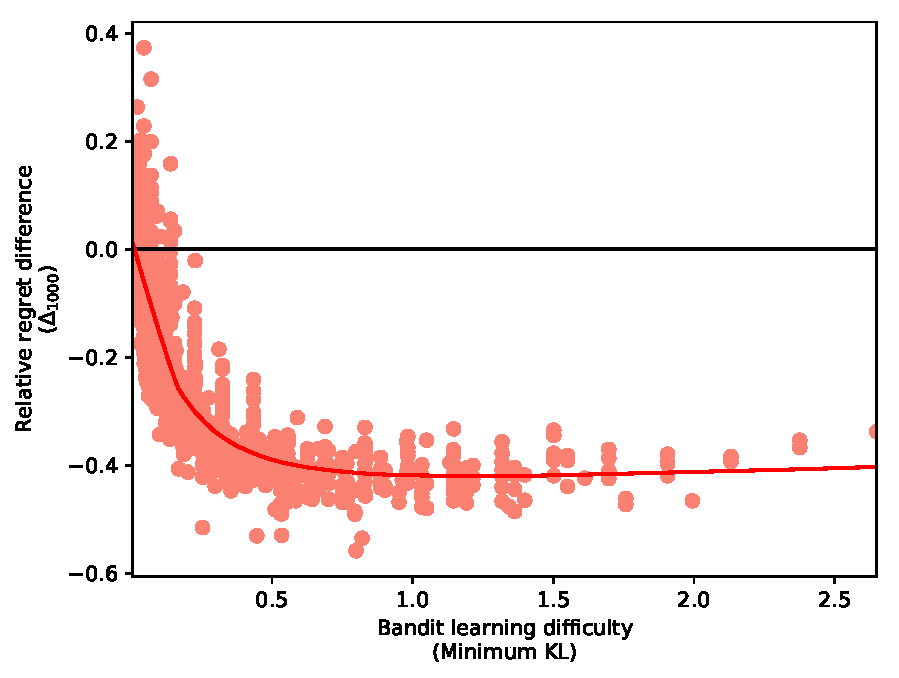
\includegraphics[width=0.5\textwidth]{./figs/bernoulli/min_KL_relDiff_t1000_07.pdf}
	\caption{Relative average expected reward differences at $t=1000$.}
	\label{fig:bernoulli_relative_cumregret_kl}
\end{figure}

\subsection{Contextual linear Gaussian bandits}
\label{ssec:contextLinearGaussian_bandits}

Another set of well studied bandits are those with continuous reward functions. It is interesting to consider the contextual case as well, where the reward distribution of each arm is dependent on a time-varying $d$-dimensional context vector. The contextual linear Gaussian bandit model is suited for these scenarios, where the expected reward of each arm is linearly dependent on the context $x\in\Real^{d}$, and the idiosyncratic parameters of the bandit $\theta\equiv\{w, \sigma\}$,
\begin{equation}
f_a(y|x,\theta)=\N(y|x^\top w_a, \sigma_a^2) \; .
\end{equation}
For this reward distribution, the posterior can be computed with the Normal Inverse Gamma conjugate prior distribution
\begin{equation}
\begin{split}
f(w_a, \sigma_a^2|u_{a,0}, V_{a,0},\alpha_{a,0}, \beta_{a,0}) &=\NIG(w_a, \sigma_a^2|u_{a,0}, V_{a,0},\alpha_{a,0}, \beta_{a,0}) \\
&= \N(w_a|u_{a,0}, \sigma_a^2 V_{a,0}) \cdot \Gamma^{-1}(\sigma_a^2|\alpha_{a,0}, \beta_{a,0}) \;, \\
\end{split}
\end{equation}
that yields, given previous actions $a_{1:t}$, contexts $x_{1:t}$ and rewards $y_{1:t}$, the following posterior
\begin{equation}\begin{split}
& f(w_a, \sigma_a^2|a_{1:t},y_{1:t},u_{a,0}, V_{a,0},\alpha_{a,0}, \beta_{a,0}) =\NIG(w_a, \sigma_a^2|u_{a,t}, V_{a,t},\alpha_{a,t}, \beta_{a,t}) \; ,\\
& \qquad \text{with} \begin{cases}
\text{sequential updates} \begin{cases}
V_{a,t}^{-1} = V_{a,t-1}^{-1} + x_t x_t^\top \cdot \mathbbm{1}[a_t=a]\\
u_{a,t}= V_{a,t} \left( V_{a,t-1}^{-1} u_{a,t-1} + x_t y_{t}\cdot \mathbbm{1}[a_t=a]\right) \\
\alpha_{a,t}=\alpha_{a,t-1} + \frac{\mathbbm{1}[a_t=a]}{2} \\
\beta_{a,t}=\beta_{a,t-1} + \frac{\mathbbm{1}[a_t=a](y_{t_a}-x_t^\top\theta_{a,t-1})^2}{2\left(1+x_t^\top \Sigma_{a,t-1} x_t\right)}
\end{cases} \\
\text{batch updates} \qquad \begin{cases}
V_{a,t}^{-1}= V_{a,0}^{-1}+x_{{1:t}|t_a} x_{{1:t}|t_a}^\top\\
u_{a,t}=V_{a,t}\left(V_{a,0}^{-1}u_{a,0}+x_{{1:t}|t_a} y_{{1:t}|t_a}\right)\\
\alpha_{a,t}=\alpha_{a,0} + \frac{|t_a|}{2} \\
\beta_{a,t}=\beta_{a,0} + \frac{\left(y_{{1:t}|t_a}^\top y_{{1:t}|t_a} + u_{a,0}^\top V_{a,0}^{-1}u_{a,0} - u_{a,t}^\top V_{a,t}^{-1}u_{a,t} \right)}{2} 
\end{cases}
\end{cases}
\end{split}
\end{equation}
where $t_a=\{t|a_t=a\}$ indicates the set of time instances when arm $a$ is played.

We provide results in Fig. \ref{fig:linearGaussian_cumulative_regret_compare} for the two-armed contextual Gaussian bandit with uniformly distributed random uncorrelated context, \ie $x_{i,t}\sim \U(0,1), i \in \{1, \cdots, d\}, t \in \Natural$. When the arms' reward distributions are comparable, our method performs similar to the Thompson sampling approach (see Fig. \ref{fig:linearGaussian_cumulative_regret_notgreat}). However, when the difference between arms is easier to learn (as in Fig. \ref{fig:linearGaussian_cumulative_regret_great}), double sampling attains reduced cumulative regret.

% Linear Gaussian: comparison of cumulative regret cases
\begin{figure}[!h]
	\centering
	\begin{subfigure}[b]{0.5\textwidth}
		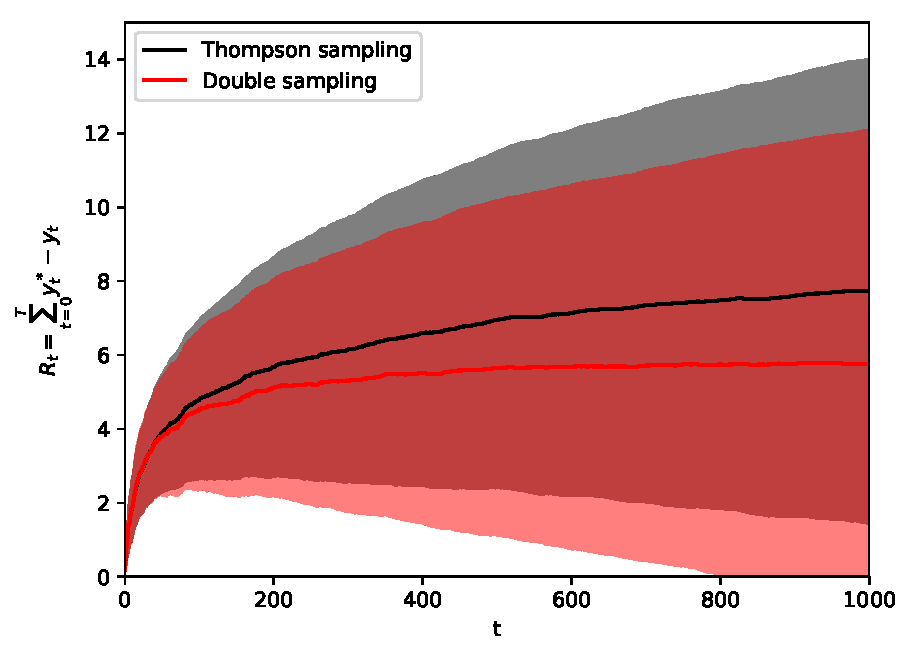
\includegraphics[width=\textwidth]{./figs/linearGaussian/cumulative_regret_great.pdf}
		\caption{Averaged cumulative regret with $A=2$, \\ $w_0=(0.4 \; 0.4)^\top$, $w_1=(0.8 \; 0.8)^\top$, $\sigma_0=\sigma_1=0.2$.}
		\label{fig:linearGaussian_cumulative_regret_great}
	\end{subfigure}%
	%add desired spacing between images, e. g. ~, \quad, \qquad etc.
	%(or a blank line to force the subfigure onto a new line)
	\begin{subfigure}[b]{0.5\textwidth}
		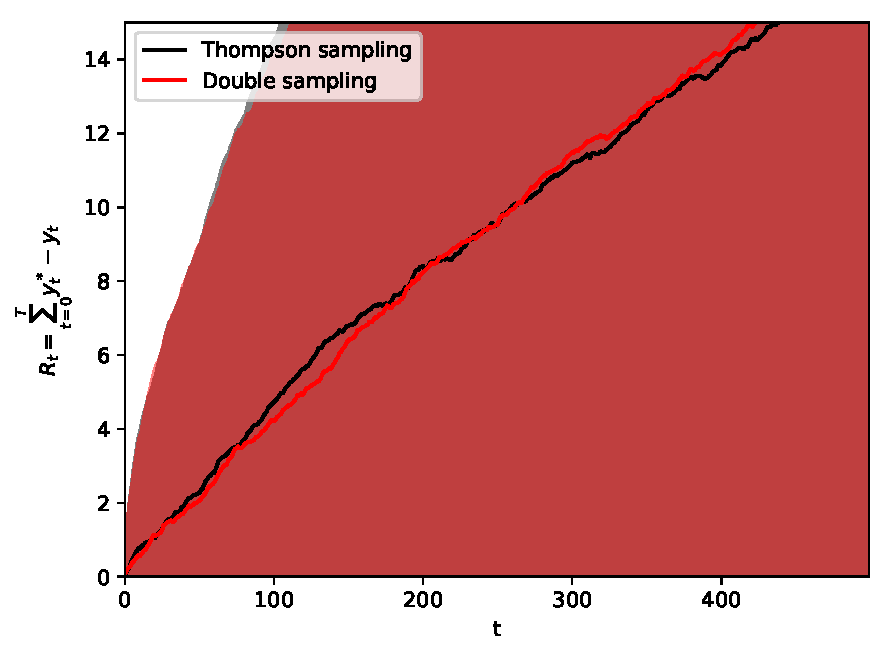
\includegraphics[width=\textwidth]{./figs/linearGaussian/cumulative_regret_notgreat.pdf}
		\caption{Averaged cumulative regret with $A=2$, \\ $w_0=(0.4 \; 0.4)^\top$, $w_1=(0.5 \; 0.5)^\top$, $\sigma_0=\sigma_1=1$.}
		\label{fig:linearGaussian_cumulative_regret_notgreat}
	\end{subfigure}
	\caption{Averaged cumulative regret comparison (standard deviation shown as shaded region).}
	\label{fig:linearGaussian_cumulative_regret_compare}
\end{figure}

We elaborate on the power of the proposed double sampling technique by evaluating the relative difference between the averaged expected rewards of our algorithm and Thompson sampling, with respect to the Kullback-Leibler divergence. 
Fig. \ref{fig:linearGaussian_relative_cumregret_kl} contains average results over 5000 realizations of the two-dimensional contextual linear Gaussian bandit with two arms, for per-dimension parameter combinations in the range $[-1,1]$ with step size $0.1$. We observe that double sampling can provide significant regret reductions for all the parameterizations of the two-armed contextual linear Gaussian bandit.

%Linear Gaussian: KL vs relative cumregret
\begin{figure}[!h]
	\centering
	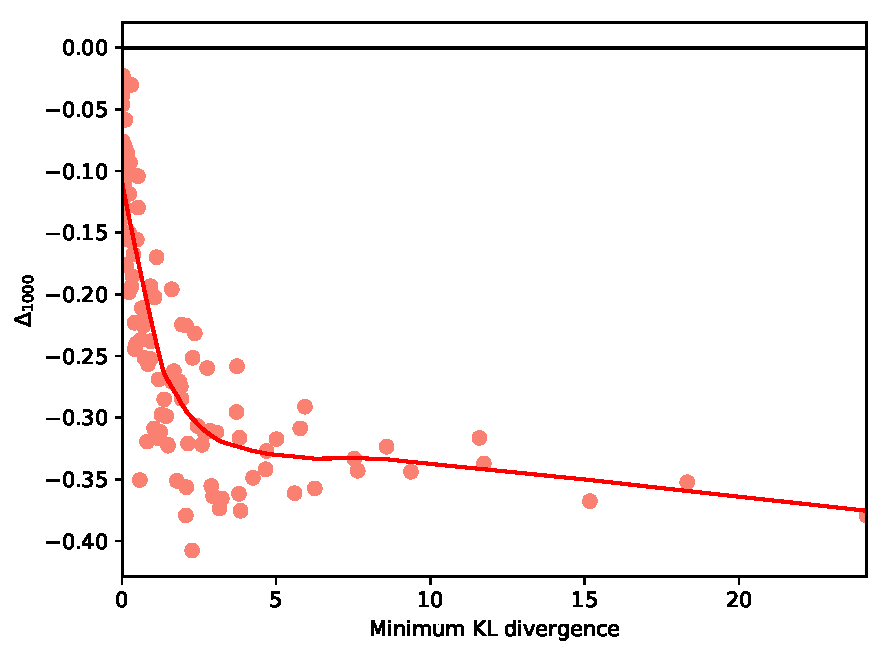
\includegraphics[width=0.5\textwidth]{./figs/linearGaussian/min_KL_relDiff_t1000_07.pdf}
	\caption{Relative average expected reward differences at $t=1000$.}
	\label{fig:linearGaussian_relative_cumregret_kl}
\end{figure}

%\subsubsection*{Acknowledgments}
%
%Use unnumbered third level headings for the acknowledgments. All
%acknowledgments go at the end of the paper. Do not include
%acknowledgments in the anonymized submission, only in the final paper.

\section{Conclusion}
\label{sec:conclusion}

We have presented a new sampling-based probability matching technique for the multi-armed bandit setting. We formulated the problem as a Bayesian sequential learning one, and leveraged random sampling to overcome two of its main challenges: approximating the analytically unsolvable integrals, and automatically balancing the exploration-exploitation tradeoff. We empirically show that additional sampling from the model can provide improved regrets, which is in many application domains inexpensive in comparison with interacting with the world. Encouraged by these findings, we aim at extending this technique to other reward distributions and implementing it with 
%real datasets.
datasets from domain application in which actions are expensive relative to samples drawn from the current model.

% Select a .bst file for the style
\bibliographystyle{plainnat}

% Generate bibliography from the specified bibliography file
\bibliography{../literature}

\end{document}
